\begin{wrapfigure}[10]{r}[0pt]{100mm}
	\centering
    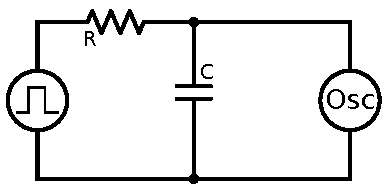
\includegraphics[width=80mm]{schema.pdf}
    \caption{Schema del circuito utilizzato.}
    \label{fig:circuito}
\end{wrapfigure}


\section{Strumenti}
%\begin{tabular}{|cc}
%$\bullet \quad$Oscilloscopio & \multirow{6}{*}{\begin{figure}
%											%	\centering
%											    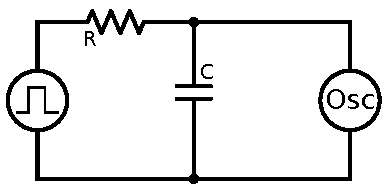
\includegraphics[scale=1]{schema.pdf}
%											    \caption{Schema del circuito utilizzato.}
%											    \label{fig:circuito}
%											\end{figure}
%											} \\


$\bullet \quad$Oscilloscopio \\
$\bullet \quad$Cablaggio\\
$\bullet \quad$Decadi di resistenze e capacità\\
$\bullet \quad$Generatore di forme d'onda\\
$\bullet \quad$Multimetro digitale\\
$\bullet \quad$Breadboard (basetta sperimentale)\\
%\end{tabular}
%\hspace{2pt}\\

\section{Preparazione circuito}

Inizialmente abbiamo collegato il generatore di forme d'onda all'oscilloscopio (uscita 1) per ottenere la forma d'onda con cui confrontare quella in output dal circuito.
In seguito è stato preparato il circuito come rappresentato in Fig. \ref{fig:circuito}.

La resistenza e il condensatore usati sono in realtà \textit{decadi di resistenze} e \textit{decadi di condensatori}. Questi oggetti sono delle scatole formate rispettivamente da diverse resistenze in serie e condensatori in parallelo. Attraverso varie manopole è possibile cambiare la loro configurazione circuitale interna, così da ottenere valori di capacità e resistenze diverse. 

\section{Parametri dell'oscilloscopio e del generatore di forme d'onda}

Una volta collegato il circuito all'oscilloscopio abbiamo dovuto tarare le scale con cui esso leggeva i dati in input e alcuni parametri con cui il generatore d'onda immetteva nel circuito la sua differenza di potenziale. Lo studio della costante di tempo $\tau$ infatti richiede che il condensatore si carichi (o scarichi) completamente prima che il valore di tensione fornita dal generatore cambi. Per questo motivo si è scelto di produrre un'onda quadra con ampiezza di 1.000 Vpp (Volt picco picco) e abbiamo settato adeguatamente l'offset %a $0.500\si{\volt}$ (?)
in modo da ottenere un'onda con $V_{min}=0\,\si{\volt}$ e $V_{max}=1\,\si{\volt}$. Utilizzando il comando \textit{trigger} si è dunque cercato di stabilizzare l'immagine della forma d'onda mostrata a schermo. Una volta fatto ciò, sono state allineate sullo schermo le forme d'onda dei due segnali, quello proveniente dal generatore e quello uscente dal circuito. Così facendo è stato possibile osservare le diversità tra i 2 segnali e analizzarli nel modo che verrà descritto nella prossima sezione.
 